\subsection{Magnetisation pools}
\label{subsec:noah__magpools}

Having dealt with this relatively dry material, I now turn to exactly how NOAH supersequences are constructed.
Ordinarily, if the recovery delay is removed from an NMR experiment, its sensitivity will be greatly reduced because insufficient magnetisation will have recovered between repetitions; or in other words, $A^{(i)}$ will be very small.
Such experiments would only really be useful if sensitivity was greatly abundant.

\begin{figure}[!ht]
    \centering
    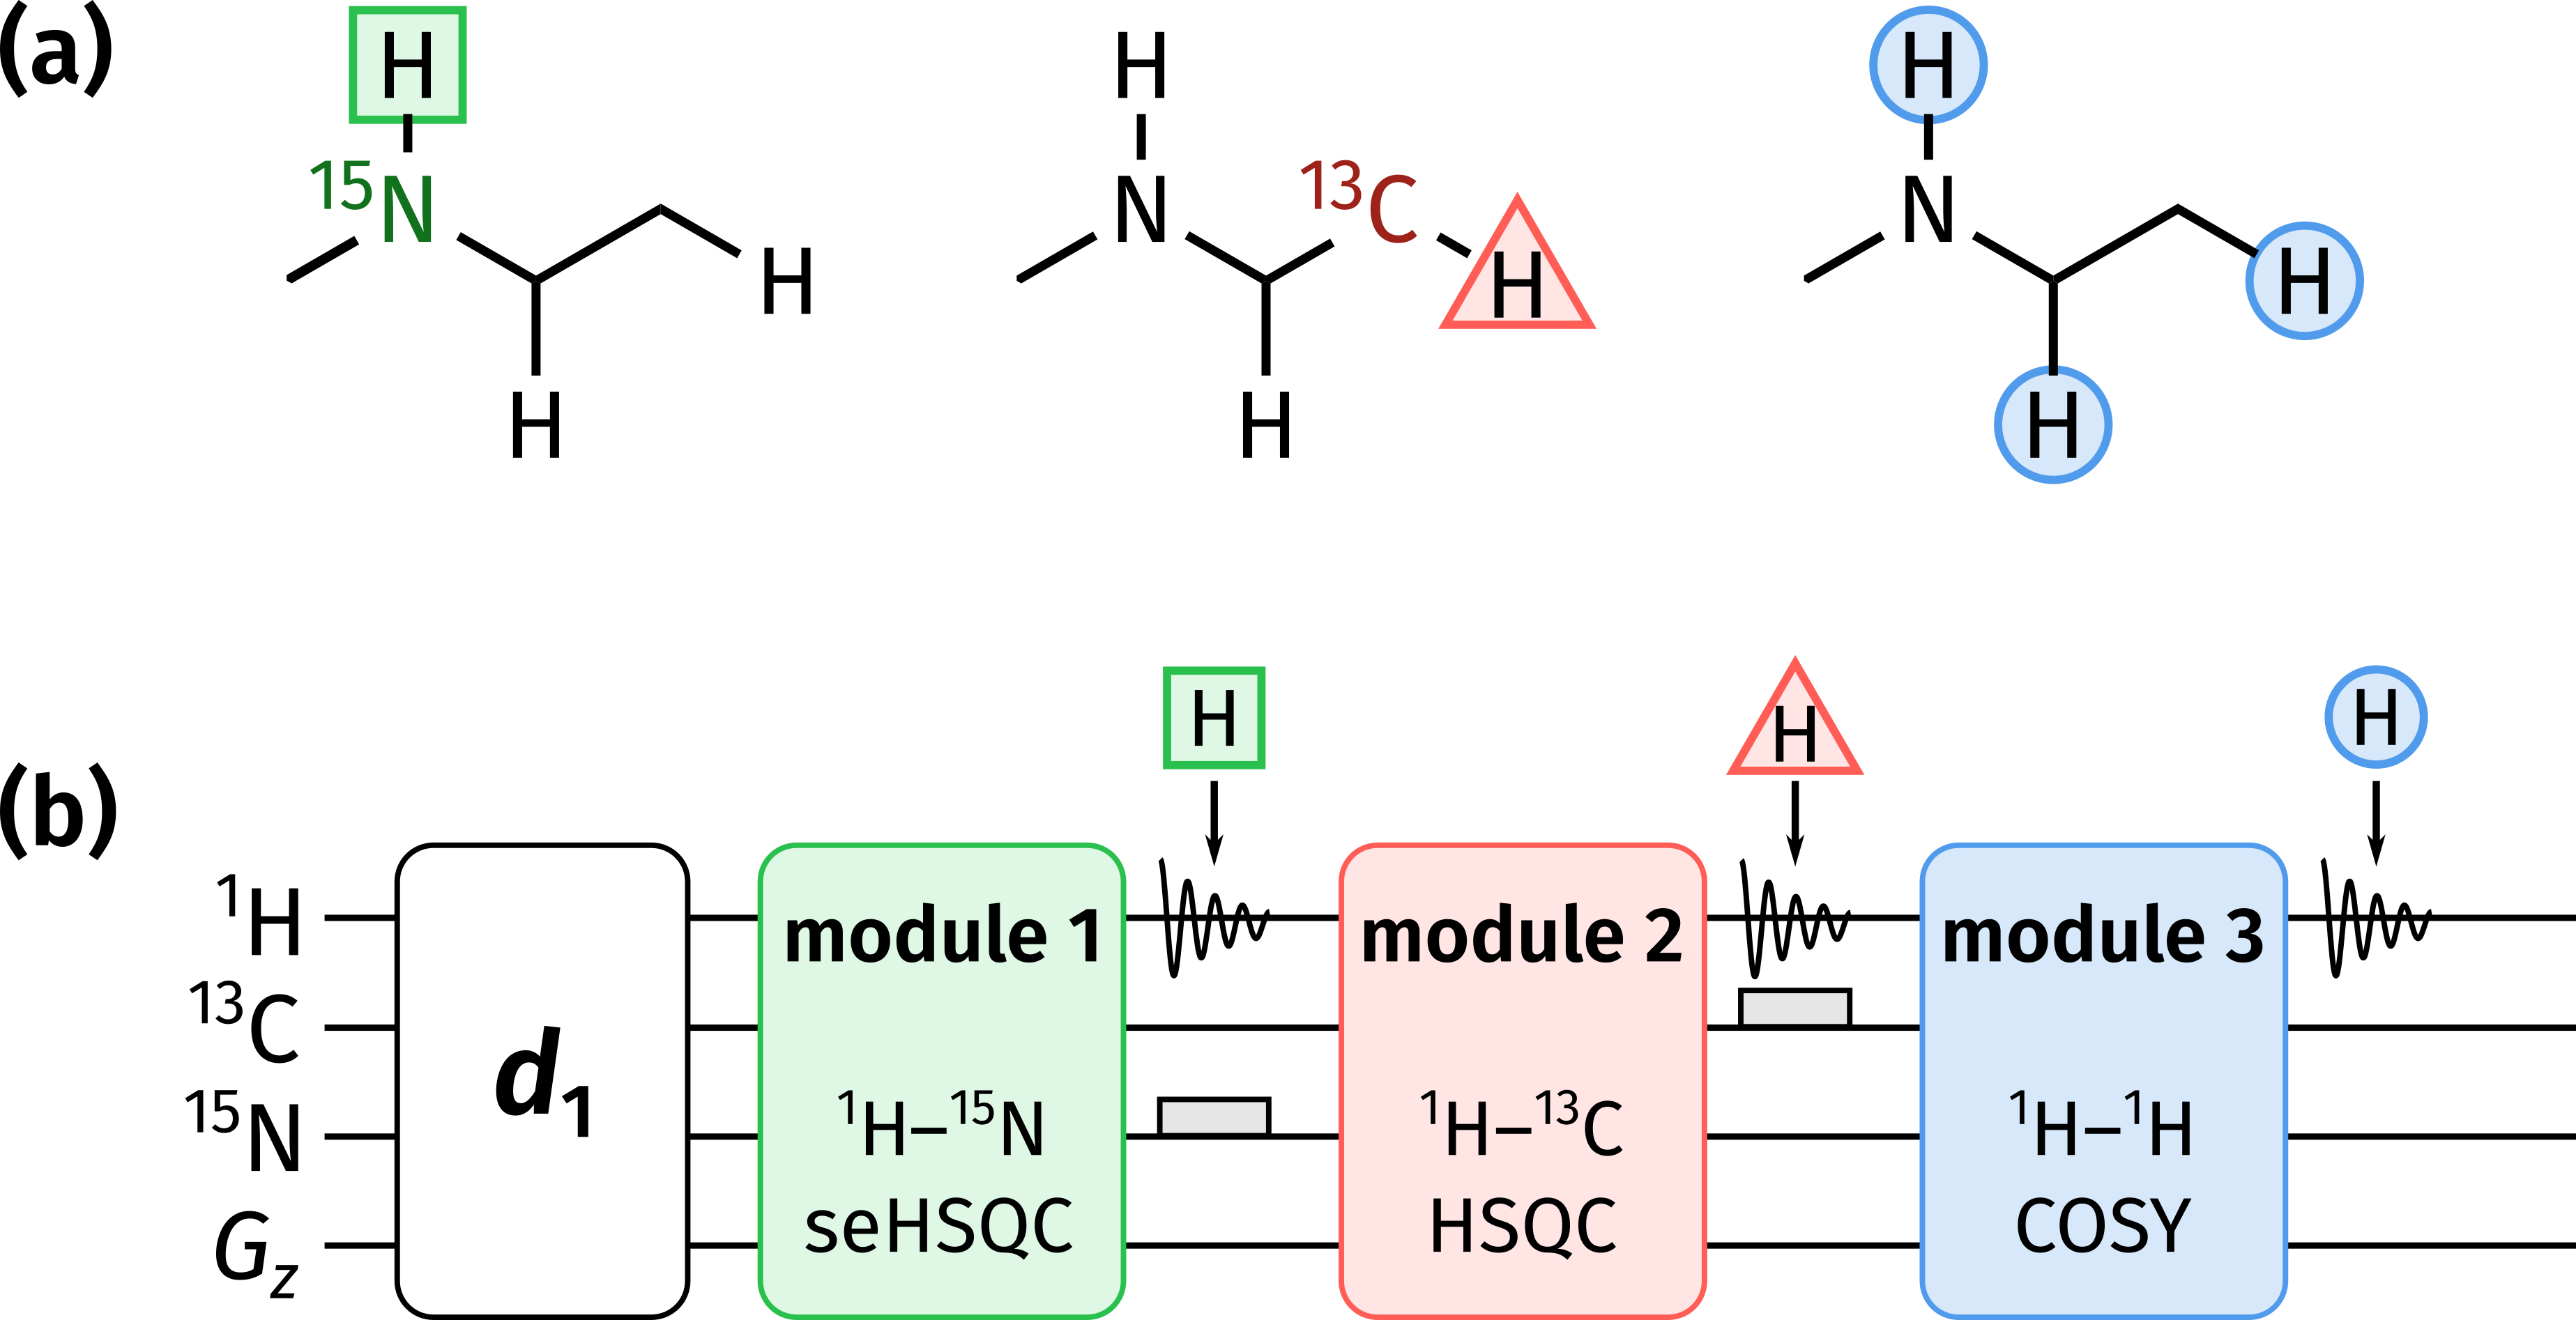
\includegraphics[]{noah/magpools.png}%
    {\phantomsubcaption\label{fig:magpools_magpools}}%
    {\phantomsubcaption\label{fig:magpools_sequences}}%
    \caption[Different magnetisation pools used in a typical NOAH supersequence]{
        \textbf{(\subref*{fig:magpools_magpools})} An illustration of the different magnetisation pools used in a typical NOAH supersequence: the three pools here (\nitrogen{}-bound protons, \carbon{}-bound protons, and all others) would be referred to as \magn{N}, \magn{C}, and \magnnot{X} respectively.
        \textbf{(\subref*{fig:magpools_sequences})} A NOAH supersequence consisting of three modules, which each consume one of the above magnetisation pools.
    }
    \label{fig:magpools}
\end{figure}

As briefly mentioned earlier, the key to avoiding this in NOAH supersequences is to make sure that \textit{each module samples a different source of magnetisation}.
These are referred to as \textit{magnetisation pools}, and arise because of the different isotopologues present in natural-abundance samples (\cref{fig:magpools_magpools}).
For example, an HSQC module can be designed to only sample magnetisation of protons directly bonded to the 1.1\%-natural abundance \carbon{}, and leave all other proton magnetisation untouched.
Immediately following this, the remainder of the proton magnetisation can then be used to record (say) a COSY module, without needing a separate recovery delay.
\Cref{fig:magpools_sequences} shows a more elaborate example, which includes both \nitrogen{} and \carbon{} HSQC experiments.

Using the notation of Orts and Gossert\autocite{Orts2018M}, the magnetisation of \carbon{}--bound protons is denoted as \magn{C}, and that of \nitrogen{}-bound protons is \magn{N}.
The magnetisation of protons \textit{not} bonded to \carbon{} is denoted as \magnnot{C} (and likewise \magnnot{N}).
Protons not directly bonded to \textit{any} NMR-active heteronucleus are labelled \magnnot{X}, and are often referred to as `bulk' magnetisation, since the majority of protons in natural-abundance samples fall into this category.

Since standard 2D experiments typically seek to \textit{destroy}---instead of \textit{preserve}---unused magnetisation, NOAH modules often require some modifications compared to standard experiments.
For example, compared to the echo--antiecho HSQC (discussed in \cref{subsec:theory__hsqc_ea}), the NOAH HSQC module\autocite{Kupce2017ACIE} adds an extra CTP gradient.
This ensures that the bulk magnetisation is refocused after $t_1$, and ultimately returned to the $+z$ equilibrium state (\cref{fig:noah_sb_po_s}).
(This is largely identical to the `symmetrised' ASAP-HSQC experiment\autocite{SchulzeSunninghausen2017JMR}.)
Sometimes, the modifications required are more extensive, such as in the HMBC module.
In order for this module to preserve \magn{C} magnetisation (e.g.\ for a later HSQC module), the initial \ang{90} excitation pulse must be replaced with a $zz$-filter (\cref{fig:noah_sb_po_b}).
This performs an \textit{isotope-selective rotation} in that \magn{C} magnetisation is stored along the $z$-axis, but \magnnot{C} magnetisation is excited and subsequently detected.

\begin{figure}[htb]
    \centering
    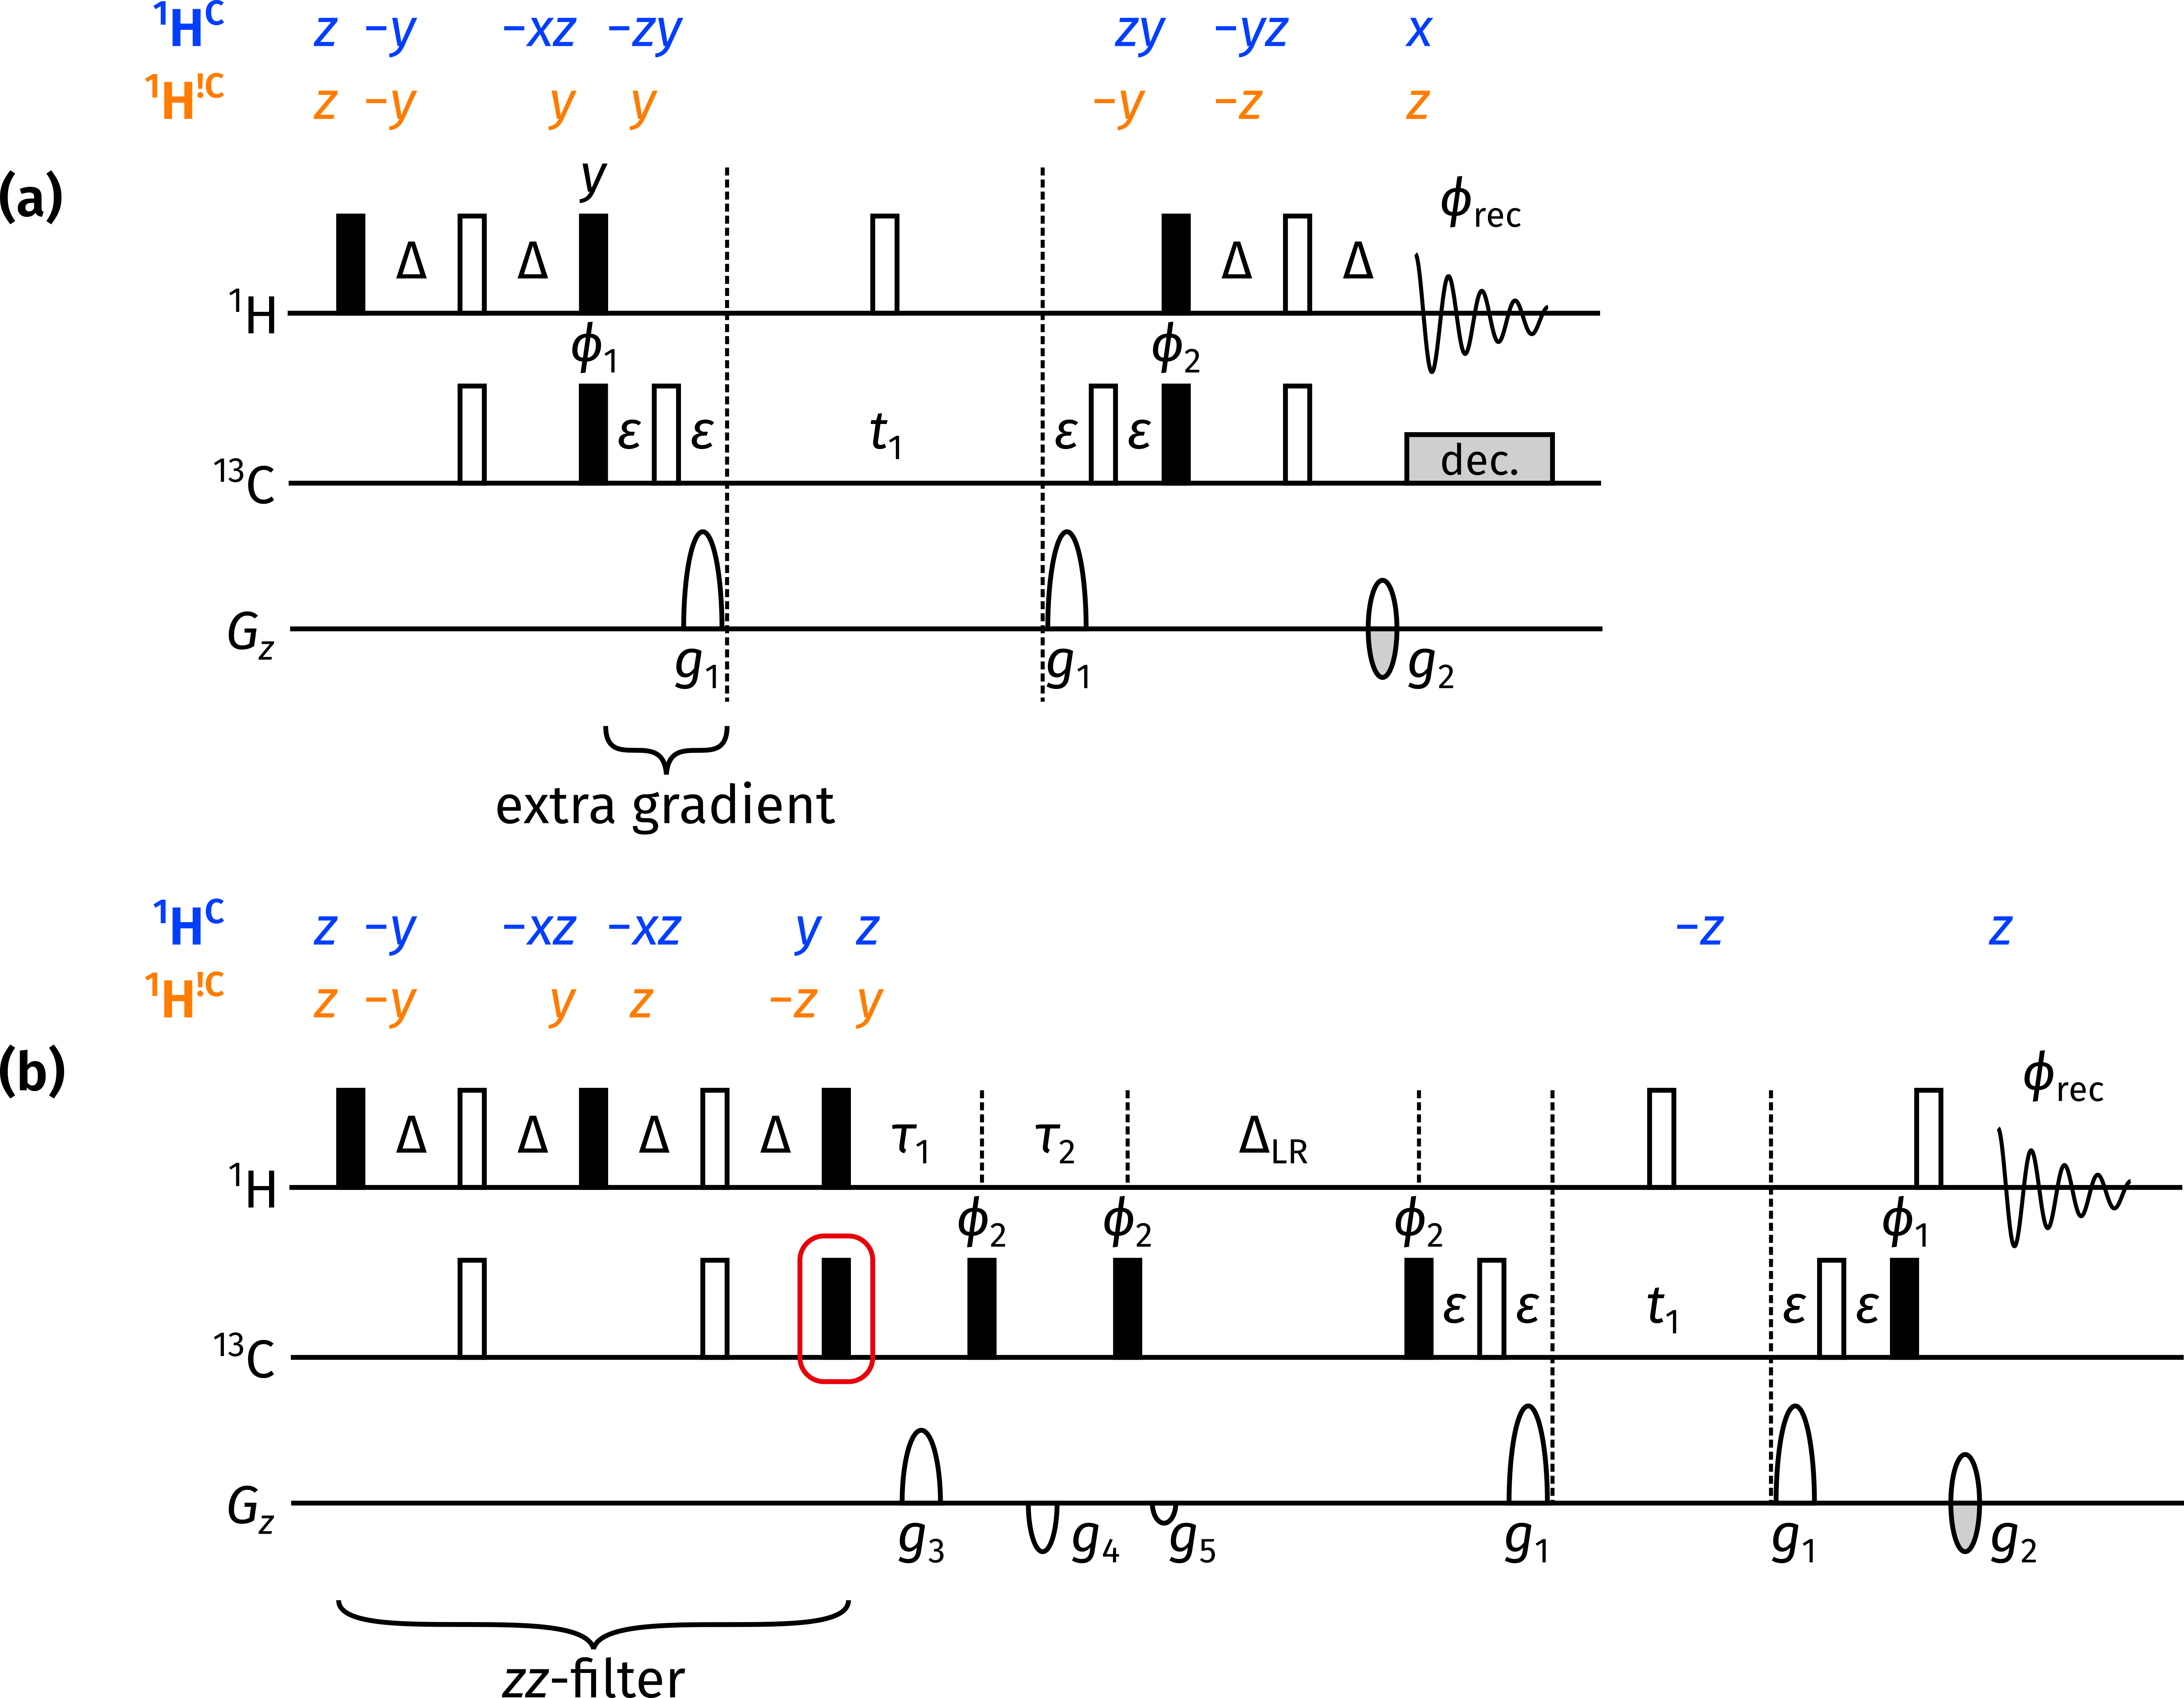
\includegraphics[]{noah/hsqc_hmbc_prodops.png}%
    {\phantomsubcaption\label{fig:noah_sb_po_s}}%
    {\phantomsubcaption\label{fig:noah_sb_po_b}}%
    \caption[NOAH HSQC and HMBC modules with product operator analysis]{
        \textbf{(\subref*{fig:noah_sb_po_s})} 
        NOAH HSQC module.
        \textbf{(\subref*{fig:noah_sb_po_b})} 
        NOAH HMBC module.
        The \ang{90} pulse highlighted in red is described in \cref{subsec:noah__hmbc}.
        Delays are set as: $\Delta = 1 / (4 \cdot \oneJ{CH})$; $\Delta_\text{LR} = 1 / (2 \cdot \nJ{CH})$; $\tau_1 = 1 / (2 \cdot \oneJ{CH,\text{max}})$; $\tau_2 = 1 / (2 \cdot \oneJ{CH,\text{min}})$ (see also \cref{subsec:poise__hmbc} for the LPJF).
        Phase cycling is performed with $\phi_1 = (x, -x)$, $\phi_2 = (x, x, -x, -x)$, and $\phi_\text{rec} = (x, -x, -x, x)$.
        Gradient amplitudes are $(g_1, g_2, g_3, g_4, g_5) = (80\%, \pm 40.2\%, 15\%, -10\%, -5\%)$.
        Product operator analysis is provided above both modules for both the \magn{C} and \magnnot{C} magnetisation pools; the notation for this is explained in the \textit{Preface}.
    }
    \label{fig:noah_sb_po}
\end{figure}

In general, sequences which are thus modified have lower sensitivities (i.e.\ $A < 1$) than the `original' sequences from which they were derived.
This is partly because of imperfect manipulation of magnetisation by the extra pulse sequence elements, and also increased losses due to relaxation during these extended sequences.
In contrast, modules placed towards the \textit{end} of a supersequence do not need to be modified, as they do not need to preserve any magnetisation.
This includes virtually all homonuclear modules, which are allowed to simply consume any remaining magnetisation.
Although this makes their implementation very straightforward, in general these modules will \textit{also} suffer some losses in sensitivity, because the preceding modules do not perfectly retain all magnetisation.

It is therefore fairly rare for a NOAH module to have $A = 1$: for this to happen, the module must be placed first in the supersequence \textit{and} not have undergone any modifications relative to the standalone experiment.%
\footnote{Of course, this also depends on exactly \textit{what} standalone experiment the NOAH supersequence is being compared against. Sometimes, in the literature, the NOAH experiment has been compared against its constituent modules acquired in a standalone fashion; in this case, the first module will always have $A = 1$, since by definition it is not modified. This tells us how much we gain through the act of concatenating modules, but is less meaningful in the `real world' where one is interested in how useful NOAH is relative to `typical' optimised 2D experiments.}
Such cases are very rare, and it is thus necessary to accept some decreases in $A$, which are often fairly small (on the order of 10--20\%).
For sensitive (typically homonuclear) modules, such sensitivity losses are often perfectly tolerable, as even with this sensitivity penalty they are still more intense than the other (heteronuclear) modules in the supersequence.
However, for insensitive modules, it is imperative to make sure that $A$ is not decreased by too much.
